\documentclass[conference]{IEEEtran}
\IEEEoverridecommandlockouts
% The preceding line is only needed to identify funding in the first footnote. If that is unneeded, please comment it out.
\usepackage{cite}
\usepackage{amsmath,amssymb,amsfonts}
\usepackage{algorithmic}
\usepackage{graphicx}
\usepackage{textcomp}
\usepackage{xcolor}
\def\BibTeX{{\rm B\kern-.05em{\sc i\kern-.025em b}\kern-.08em
    T\kern-.1667em\lower.7ex\hbox{E}\kern-.125emX}}
\begin{document}

\title{Practical Work: \\ Investigations on Remove and Retrain}

\author{\IEEEauthorblockN{1\textsuperscript{st} Viktor Maximilian Loreth}
\IEEEauthorblockA{\textit{Institute of Computational Perception} \\
\textit{Johannes Kepler University}\\
4040 Linz, Austria \\
viktor.loreth@protonmail.com}
}


\maketitle

\begin{abstract}
This report investigates the use of saliency maps in deep learning for image recognition and evaluates the effectiveness of the integrated gradient method for identifying important pixels in the MNIST dataset. In current deep learning models, it is often challenging to understand the decision-making process, making saliency maps a popular method for interpreting the importance of input features. "Remove and Retrain" tries to solve this problem by offering a numerical evaluation method. 
\end{abstract}


\section{Scientific Motivation and Goal}
Artificial neural networks have become increasingly complex in recent years, with the rise of deep learning leading to models with billions of parameters. These models have been successful in achieving state-of-the-art results on various tasks, including image recognition, natural language processing, and speech recognition. However, as these models become more complex, they also become more difficult to interpret. Creating accurate saliency maps is not a trivial task, particularly for complex models with many parameters. Several methods have been proposed for generating saliency maps, including gradient-based methods, perturbation-based methods, and activation-based methods. The effectiveness of these methods can vary depending on the model architecture, the input data, and the specific task. Evaluating saliency methods is not easy due to the lack of a ground truth or reference saliency map to compare against. This is because there are often multiple valid interpretations of a given input, and what might be salient to one observer may not be salient to another. Remove and Retrain is the state of the art method to evaluate saliency maps.


\subsection{Trying out various methods}

At the beginning of this project, several datasets were considered for training saliency models, including ImageNet, Food101, and MNIST. The sheer size of ImageNet\cite{ImageNet} presented significant computational challenges, as creating a baseline and altered datasets alone required saving a big amount of data. Additionally, generating saliency maps for this dataset and training the resNet50 model 50 times would have been too expensive considering the scope of the project.
 While Food101 offered a more manageable 50GB of data, generating saliency maps using resNET50\cite{ResNet50} and training the models took too long for the available hardware. Ultimately, the MNIST dataset\cite{MNIST} was selected for its ease of training, ease of creating other datasets, and the potential for rapid results.

\section{Training}

\subsection{Training the model}
The model used in this study is a simple convolutional neural network architecture consisting of two convolutional layers, two pooling layers, and three linear layers. The model was trained for ten epochs with a learning rate of 1e-3 and an SGD optimizer with a momentum term of 0.9. Across five separate runs, the model achieved an average accuracy of 98\% on the test data.

\subsection{Dataset preparation and Splitting}\label{AA}
The dataset used in this report was normalized using the mean and standard deviation, and was split using the PyTorch library's default splitting method. The cross entropy loss was selected. The same dataset split was used for all training iterations to ensure consistency in the results.

\section{Retraining on saliency maps}

\subsection{Generating the new datasets}
To evaluate the performance of various datasets, the integrated gradient method was utilized. A set of thresholds was defined, and the x\% most significant pixels were replaced with the mean value of the MNIST dataset. The saliency maps were utilized to identify the most critical pixels by evaluating their absolute values and selecting the highest ones. The implementation was done using the captum library.

\begin{enumerate}
	    \item[1.)] Replacement with the mean value
	
	To ensure that replacing a pixel is meaningful for any kind of pixel the mean value is taken. By taken any other value which is closer to black or white pixels, removing the respective pixel does not change the picture.
	
		\item[2.)] Why retraining is required
	
	One main property of machine learning is that the training data and the test data must be drawn from the same distribution. Without retraining the model this property is ignored as mentioned in \cite{RoaR}.
	
\end{enumerate}

\subsection{Retraining upon the new datasets}

To ensure that the model learns consistently, the same split and learning parameters were utilized as in the standard case to retrain the model on the new dataset. An unweighted network was created and then retrained for each training run. In order to validate the results and minimize the impact of random seed initialization, the training was performed with 5 different seeds and 5 models were created.

\section{Results}

To compare the effectiveness of the saliency map, it was compared to a random baseline, which masked x\% of the pixels randomly.

\begin{figure}[h]
	\centering
	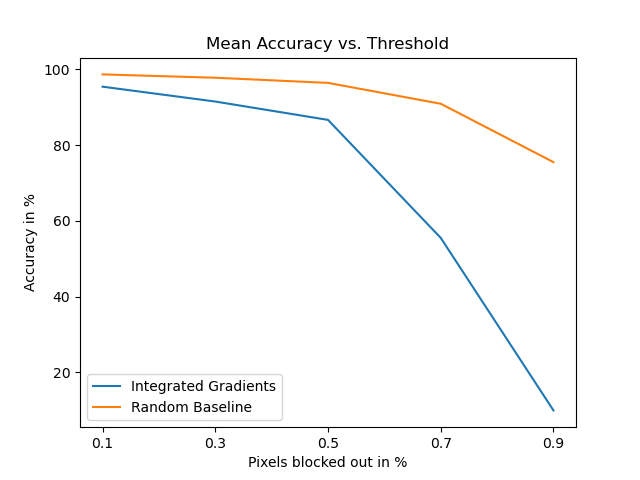
\includegraphics[width=0.5\textwidth]{figs/mean_accuracy_vs_threshold.png}
	\caption{Mean Accuracy vs Threshold}
	\label{fig:mean_accuracy}
\end{figure}

\begin{table}[ht]
	\centering
	\begin{tabular}{|c|c|c|c|c|c|}
		\hline
		Pixels removed & 10\% & 30\% & 50\% & 70\% & 90\% \\
		\hline
		Integrated Gradient & 0.44\% & 0.83\% & 2.10\% & 31.64\% & 0\% \\
		Random Baseline  & 0.42\% & 0.28\% & 0.39\% & 0.58\% & 0.65\% \\
		\hline	
	\end{tabular} \newline
	
	\caption{Standard deviation of mean accuracy over 5 Training runs}
	\label{tab:std_deviation}
\end{table}

In this plot one can see that Integrated Gradients learns significantly worse than the Random Baseline and at 90\% of the pixels removed the performance is as good as a random guess: 10\%.



\subsection{Interpretation of results}

The rising standard deviation indicates that the model is not able to learn reliably anymore. This implies that the model finds arbitrary new structures in the images which is interpreted wrongly. The learning parameters could be adapted to improve the scores, but it is clear that the accuracy is lower than in the other thresholds.
\\
In the Appendix the precision of the models are shown. For the integrated gradient method there exist a higher std deviations and lower precision, which means that the models are not able to learn reli anymore.

The RoaR method can effectively proof for the MNIST dataset if integrated gradients do indeed show important pixels. Contrary to the results in \cite{RoaR}, Integrated Gradient is successfully finding meaningful pictures. This could be due to the huge size of the ResNET50 model, but more investigation is needed to make a proper statement.


\begin{thebibliography}{00}
\bibitem{RoaR} Sara Hooker, Dumitru Erhan, Pieter-Jan Kindermans and Been Kim, ``A Benchmark for Interpretability Methods in Deep Neural Networks'' Google Brain, 33rd Conference on Neural Information Processing Systems (NeurIPS 2019), 5 Nov 2019.
\bibitem{Integrated Gradient} Mukund Sundararajan, Ankur Taly and Quiqi Yan,``Axiomatic Attribution for Deep Networks'', Proceedings of the 34 th International Conference on Machine Learning, Sydney, Australia, PMLR 70, 2017. 
\bibitem{MNIST} L. Deng, "The MNIST Database of Handwritten Digit Images for Machine Learning Research [Best of the Web]," in IEEE Signal Processing Magazine, vol. 29, no. 6, pp. 141-142, Nov. 2012, doi: 10.1109/MSP.2012.2211477.
\bibitem{ResNet50} Kaiming He, Xiangyu Zhang, Shaoqing Ren and  Jian Sun, ``Deep Residual Learning for Image Recognition'', 2016 IEEE Conference on Computer Vision and Pattern Recognition (CVPR), June 2016 
\bibitem{ImageNet} Jia Deng, Wei Dong, Richard Socher, Li-Jia Li, Kai Li and Li Fei-Fei, ``ImageNet: A Large-Scale Hierarchical Image Database'', IEEE Conference on Computer Vision and Pattern Recognition 2009
\bibitem{Food101} Lukas Bossard, Guillaumin Matthieu and Luc Van Gool, ``Food-101 -- Mining Discriminative Components with Random Forests'', IEuropean Conference on Computer Vision 2014
\end{thebibliography}
\onecolumn
\newpage



\section{Appendix}
\centering
Precision and standard deviation of the retrained models per threshold.

\begin{table}[h]
	\centering
	\begin{tabular}{|c|c|c|c|c|c|c|c|c|c|c|}
		\hline
		
		Pixels removed & 0 & 1 & 2 & 3 & 4 & 5 & 6 & 7 & 8 & 9 \\
		\hline
		10\%& 97.2 & 95.4 & 96.2 & 94.6 & 95.6 & 97.2 & 98.4 & 96.2 & 92.8 & 90.4 \\
		std & 0.98 & 0.80 & 0.98 & 1.36 & 1.62 & 2.04 & 1.50 & 2.71 & 1.83 & 3.61 \\
		\hline
		30\% &  94.6 & 95.4 & 92.4 & 87.0 & 86.2 & 91.4 & 96.2 & 92.4 & 87.8 & 91.4 \\
		std & 2.06 & 1.74 & 2.94 & 6.26 & 2.79 & 3.26 & 0.98 & 2.50 & 2.56 & 2.94 \\
		\hline
		50\% &93.8 & 89.6 & 82.6 & 85.2 & 79.0 & 92.4 & 94.2 & 88.8 & 73.8 & 87.0  \\
		std & 2.64 & 4.03 & 4.84 & 5.42 & 1.90 & 4.13 & 2.14 & 3.60 & 5.74 & 1.79 \\
		\hline
		70\% & 74.2 & 88.0 & 52.0 & 59.4 & 35.6 & 50.0 & 55.2 & 55.8 & 41.4 & 43.6  \\
		std & 37.1 & 7.5 & 38.6 & 38.8 & 30.1 & 40.9 & 45.1 & 36.0 & 34.5 & 35.6 \\
		\hline
		90\% & 0.00 & 100.00 & 0.00 & 0.00 & 0.00 & 0.00 & 0.00 & 0.00 & 0.00 & 0.00  \\
		std & 0.00 & 0.00 & 0.00 & 0.00 & 0.00 & 0.00 & 0.00 & 0.00 & 0.00 & 0.00 \\
		\hline
	\end{tabular} \newline
	
	\caption{Class Precision and Std deviation (values in \%) Integrated Gradient}
	\label{tab:sclass_precision_ig}
\end{table}



\begin{table}[h]
	\centering
	\begin{tabular}{|c|c|c|c|c|c|c|c|c|c|c|}
		\hline
		
		Pixels removed & 0 & 1 & 2 & 3 & 4 & 5 & 6 & 7 & 8 & 9 \\
		\hline
		10\%& 100.0 & 100.0 & 97.2 & 100.0 & 98.4 & 98.4 & 98.8 & 98.0 & 96.8 & 98.8 \\
		std & 0.0 & 0.0 & 0.98 & 0.0 & 0.8 & 0.8 & 0.98 & 1.26 & 1.47 & 1.60 \\ 
		\hline
		30\% &  98.4 & 99.6 & 98.0 & 98.8 & 95.2 & 98.0 & 97.6 & 97.6 & 98.4 & 96.0 \\
		std & 0.80 & 0.80 & 1.26 & 1.60 & 1.17 & 1.79 & 0.80 & 1.50 & 0.80 & 1.90 \\
		\hline
		50\% &100.0 & 96.4 & 95.0 & 96.6 & 94.2 & 97.2 & 99.2 & 95.6 & 94.8 & 95.0 \\
		std & 0.00 & 1.20 & 1.55 & 1.96 & 2.64 & 1.60 & 1.60 & 0.49 & 1.47 & 1.10 \\
		\hline
		70\% & 95.8 & 95.4 & 92.2 & 86.0 & 90.0 & 91.8 & 94.0 & 93.8 & 85.2 & 84.8 \\
		std & 1.60 & 0.80 & 3.66 & 3.95 & 2.76 & 2.32 & 1.79 & 1.47 & 3.06 & 4.87 \\
		\hline
		90\% & 87.4 & 89.2 & 85.6 & 67.6 & 56.8 & 71.4 & 85.2 & 79.8 & 68.8 & 63.2  \\
		std & 1.96 & 0.98 & 4.32 & 4.36 & 8.80 & 5.31 & 1.17 & 2.86 & 4.96 & 6.97 \\
		\hline
	\end{tabular} \newline
	
	\caption{Class Precision and Std deviation (values in \%) Random Baseline}
	\label{tab:sclass_accuracy_random}
\end{table}


% restore original margins
\vspace{12pt}
\color{red}

\end{document}
